\section{Reliability and availability}

Dependability can be subdivided into the following components:
\begin{figure}[H]
    \centering
    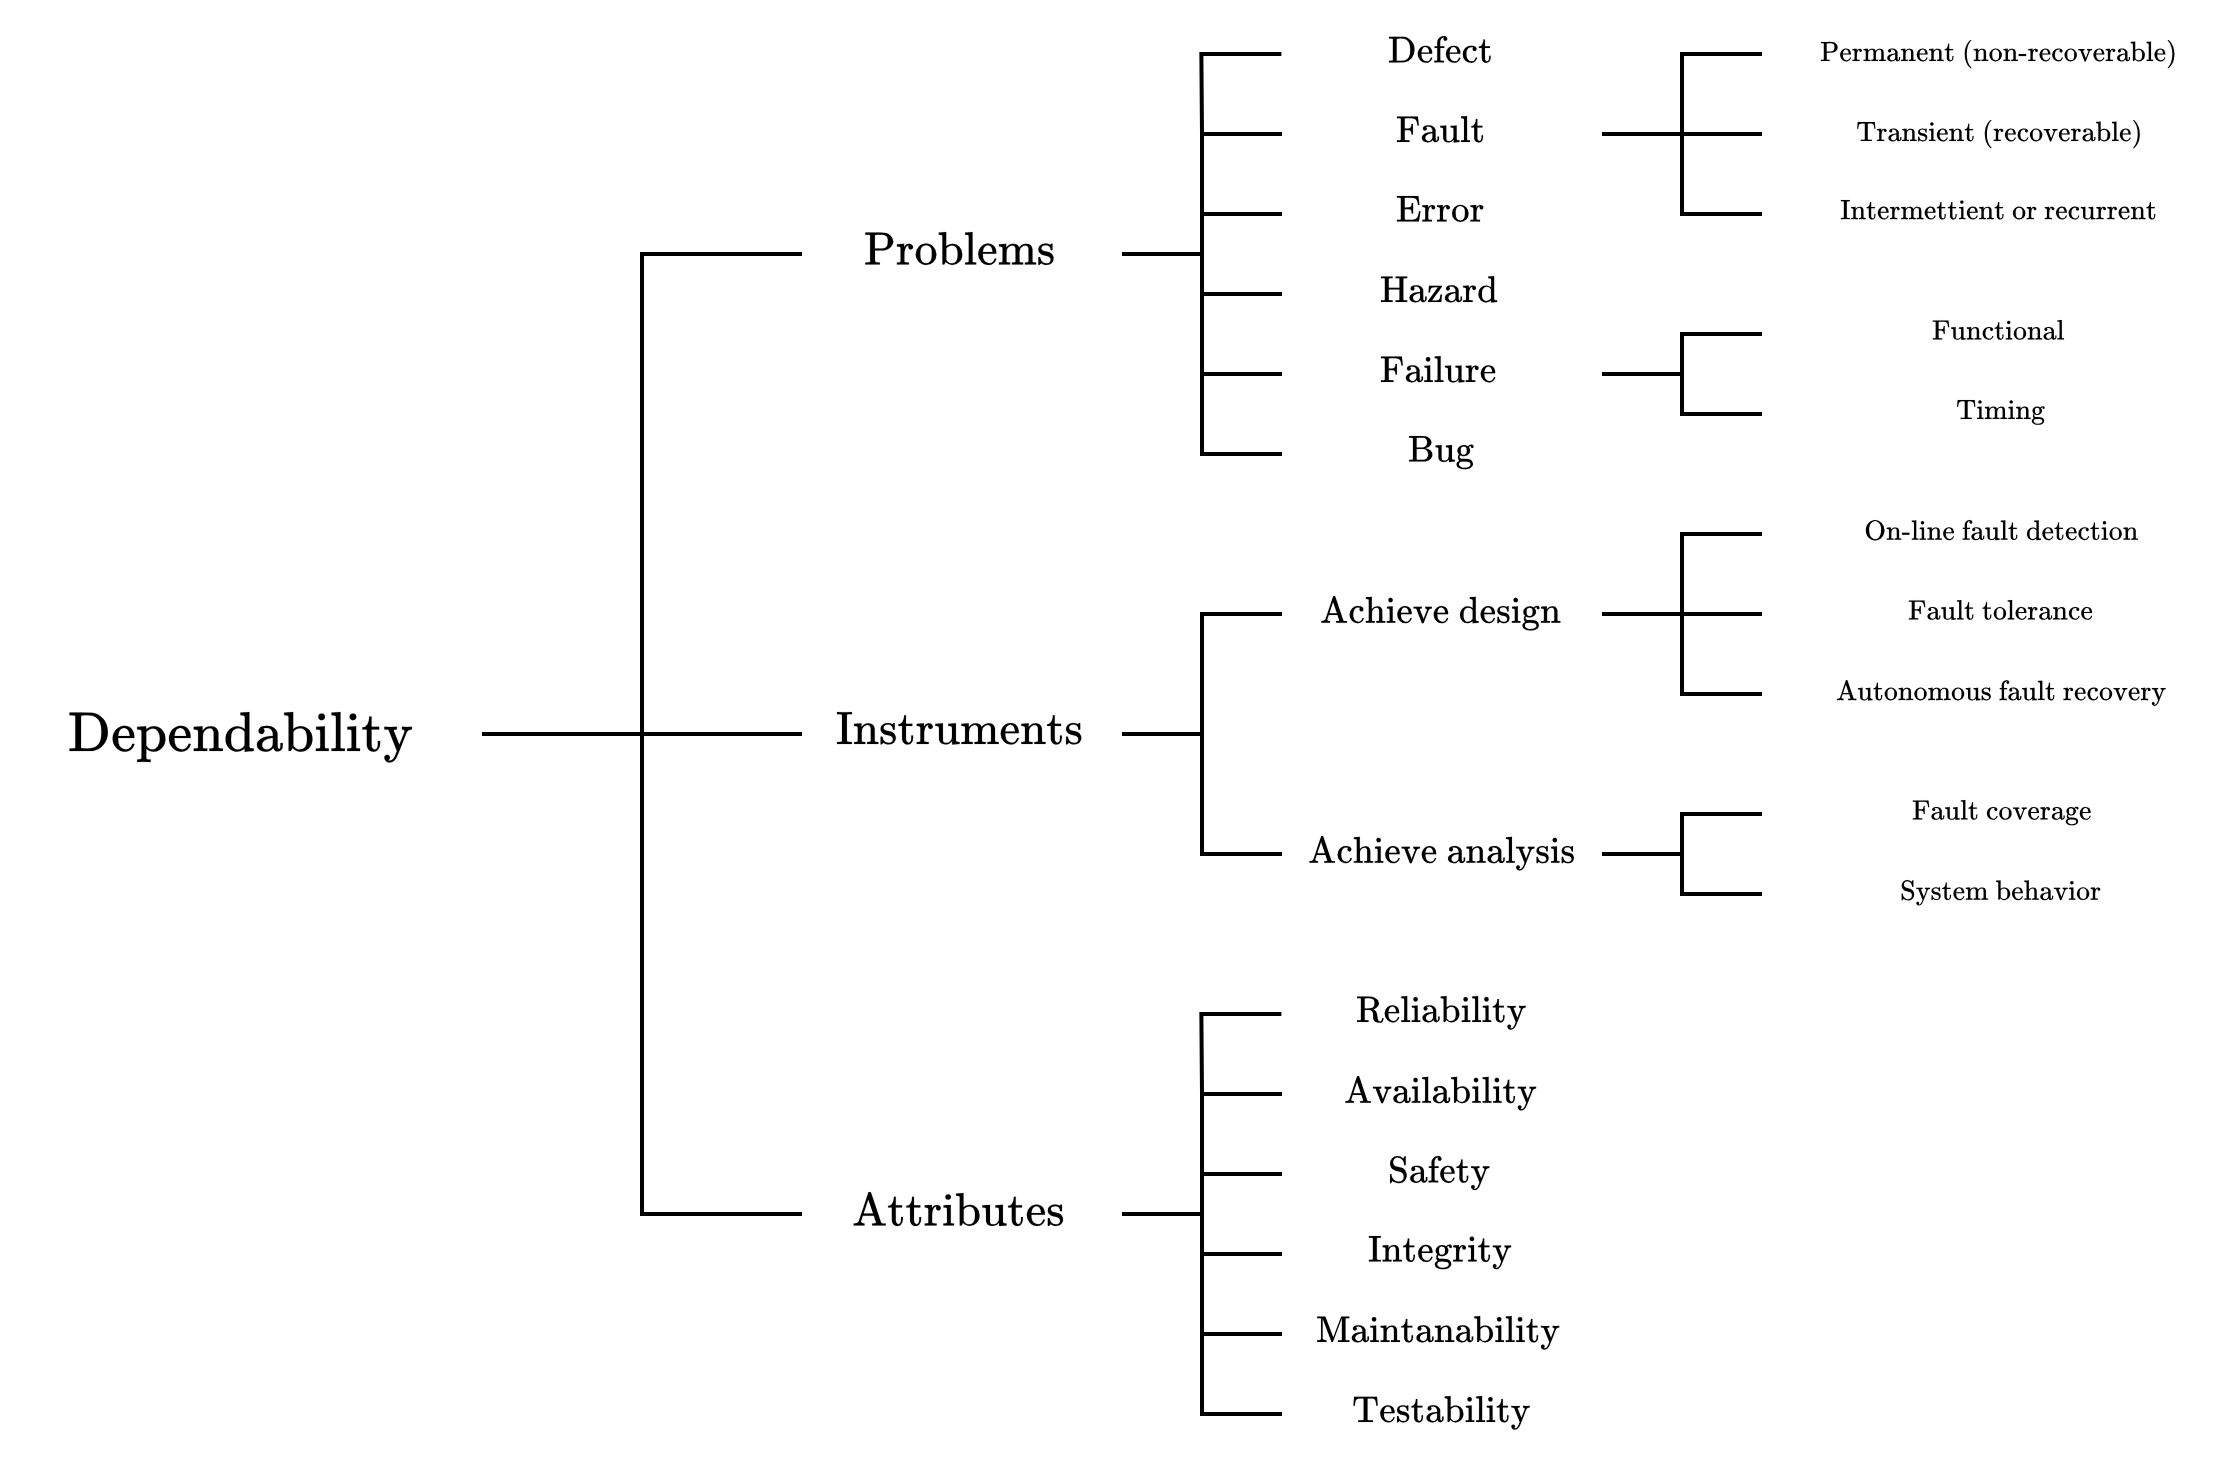
\includegraphics[width=0.6\linewidth]{images/dep1.png}
    \caption{Dependability components}
\end{figure}

\subsection{Reliability}
\begin{definition}[\textit{Reliability}]
    Reliability is the ability of a system or component to perform its required functions under stated conditions for a specified period of time. 
\end{definition}
We denote $R(t)$ as the probability of the system operating correctly in a designated environment until time $t$, expressed as:
\[R(t)=\text{P}(\text{not failed during }[0,t])\]
assuming it was operational at time $t = 0$.
If a system is required to function for ten-hour intervals, then the reliability target is set for ten hours.
$R(t)$ is a monotonically decreasing function ranging from 1 to 0 over 0 to infinity:
\[\lim_{x\rightarrow + \infty}R(t)=0\]
This metric is often applied to systems where even brief periods of malfunction are intolerable, such as those with stringent performance, timing, or safety requirements, or those that are challenging or impossible to repair.
\paragraph*{Unreliability}
The unreliability is the complementary measure to reliability and is calculated as:
\[1-R(t)\]

\subsection{Availability}
\begin{definition}[\textit{Availability}]
    Availability is the e degree to which a system or component is operational and accessible when required for use. 
\end{definition}
It is defined as: 
\[\text{Availability}=\dfrac{\text{Uptime}}{\text{Uptime}+\text{Downtime}}\]
We denote as $A(t)$ the probability that the system will be operational at time $t$: 
\[A(t)=\text{P}(\text{not failed at time }t)\]
Literally, readiness for service
Admits the possibility of brief outages
Fundamentally different from reliability
\paragraph*{Unavailability}
The unavailability is the complementary measure to availability and is calculated as:
\[1-A(t)\]
\begin{definition}[\textit{Repairable system}]
    A system is sad to be repairable if $A(t) \geq R(t)$. 
\end{definition}
\begin{definition}[\textit{Unrepairable system}]
    A system is sad to be unrepairable if $A(t) = R(t)$. 
\end{definition}

\subsection{Other indices}
\begin{definition}[\textit{Mean time to failure}]
    The mean time to failure represents the average duration before any failure occurs.
\end{definition}
\begin{definition}[\textit{Mean time between failures}]
    The mean time between failures denotes the average duration between two consecutive failures.
\end{definition}
\begin{figure}[H]
    \centering
    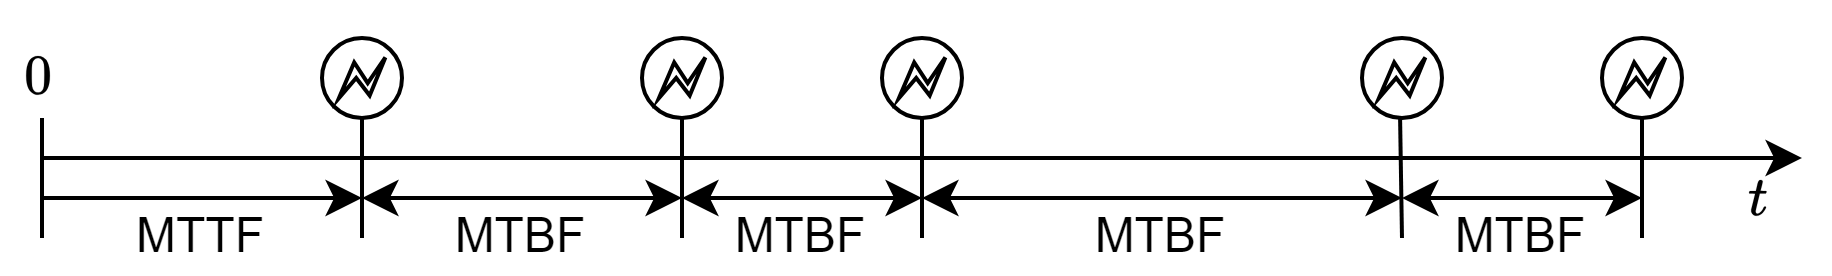
\includegraphics[width=0.75\linewidth]{images/mttb.png}
    \caption{Example of MTTF and MTBF}
\end{figure}
The MTTF can alternatively be calculated as the integral of reliability:
\[\text{MTTF}=\int_0^\infty R(t)dt\]
Additionally, the MTBF can be defined as:
\[\text{MTBF}=\dfrac{\text{total operating time}}{\text{number of failures}}\]
\begin{definition}[\textit{Failures in time}]
    Failures in time refer to the reciprocal of the mean time between failures.
\end{definition}
The failures in time, denoted as $\lambda$, are computed as:
\[\lambda=\dfrac{\text{number of failures}}{\text{total operating time}}=\dfrac{1}{\text{MTBF}}\]
Typically, it is computed based on a scale of one billion hours.
\begin{definition}[\textit{Infant mortality}]
    Infant mortality measures failures occurring in new systems, often observed during testing phases rather than during production.
\end{definition}
\begin{definition}[\textit{Random failures}]
    Random failures occur sporadically throughout the lifespan of a system.
\end{definition}
\begin{definition}[\textit{Wear out}]
    Wear out refers to the failure of components at the end of their operational life, potentially leading to system failure. 
\end{definition}
Preemptive maintenance can mitigate this type of failure.
\begin{figure}[H]
    \centering
    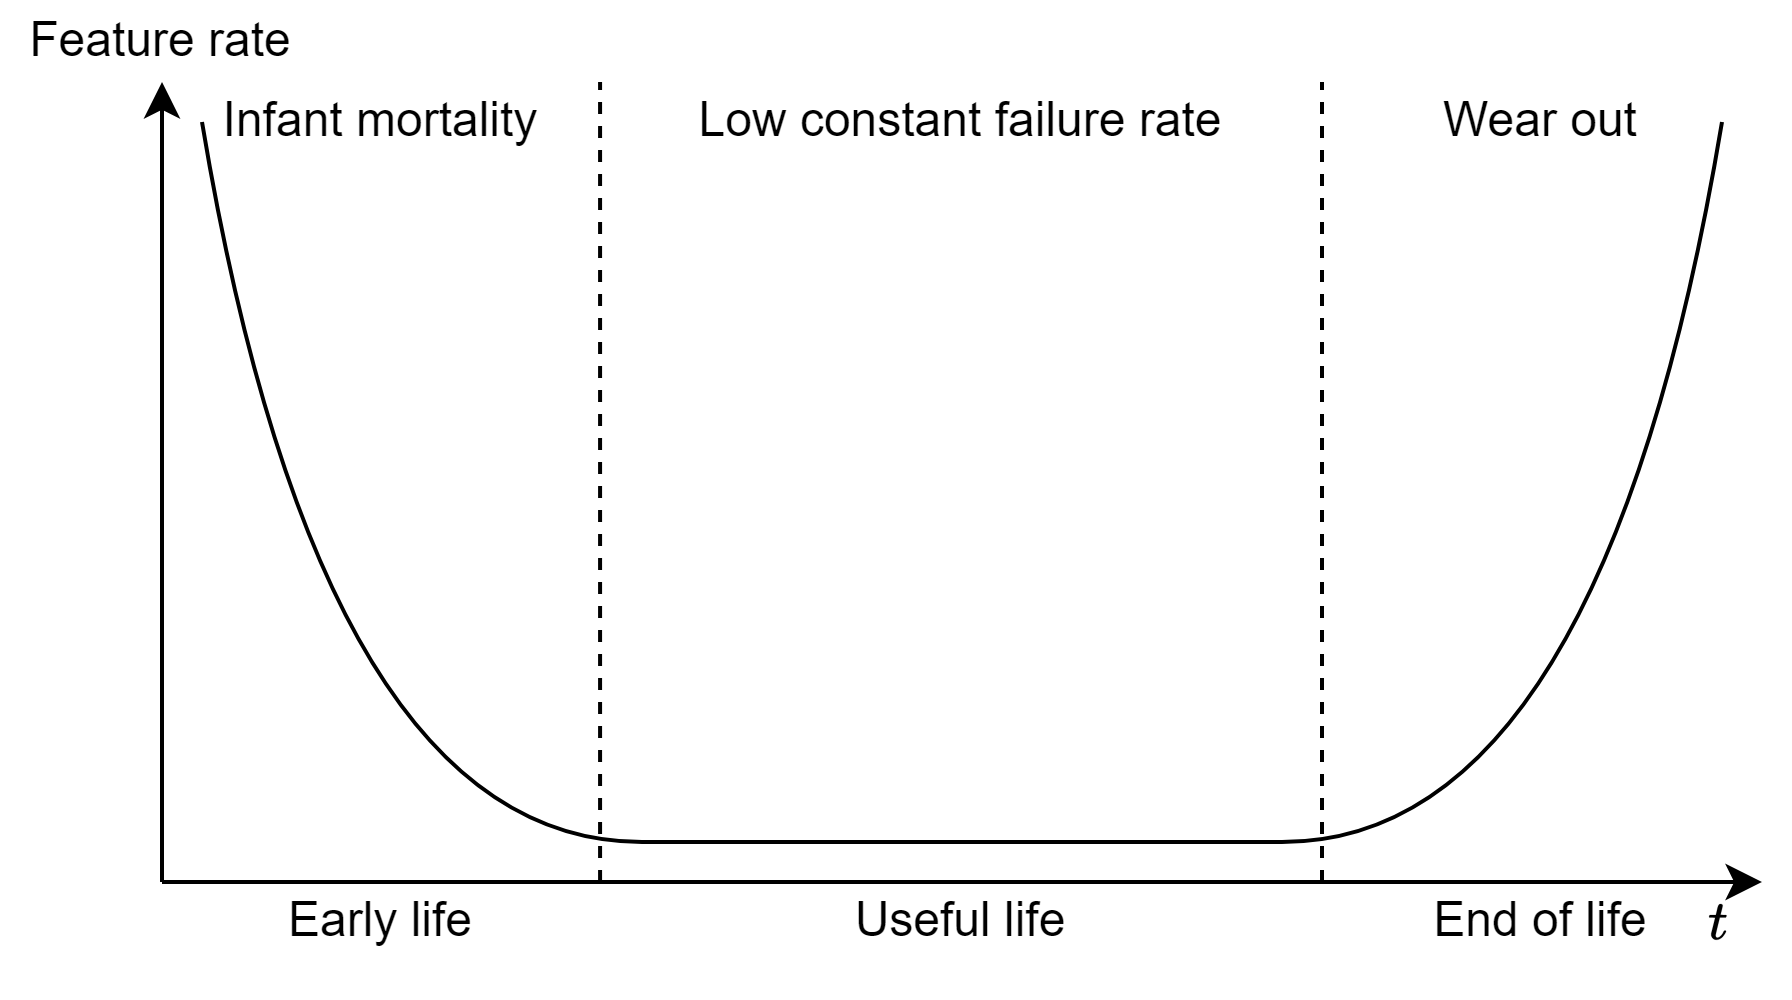
\includegraphics[width=0.55\linewidth]{images/dep2.png}
    \caption{Product reliability curve}
\end{figure}

\subsection{Defect identification}
To identify defective products and determine the Mean Time To Failure (MTTF), a burn-in test can be conducted. 
During this test, the system is subjected to elevated levels of temperature, voltage, current, and humidity to accelerate wear and tear.

In scenarios where systems exhibit low reliability but must remain operational, quick repairs of system failures that do not compromise data integrity may help mitigate the impact of low reliability. 
For example, in a database management system, low reliability might not present significant issues.

On the other hand, ensuring high reliability in systems can pose greater challenges.

Utilizing information from the reliability function $R(t)$ allows for the computation of a complex system's reliability over time, representing its expected lifetime. 
This process involves calculating the MTTF and determining the overall reliability by aggregating the reliability of individual components.

\begin{definition}[\textit{Fault}]
    A fault refers to a defect within the system.
\end{definition}
\begin{definition}[\textit{Error}]
    An error represents a deviation from the intended operation of the system or subsystem.
\end{definition}
\begin{definition}[\textit{Failure}]
    A failure occurs when the system is unable to perform its designated function.
\end{definition}
\begin{figure}[H]
    \centering
    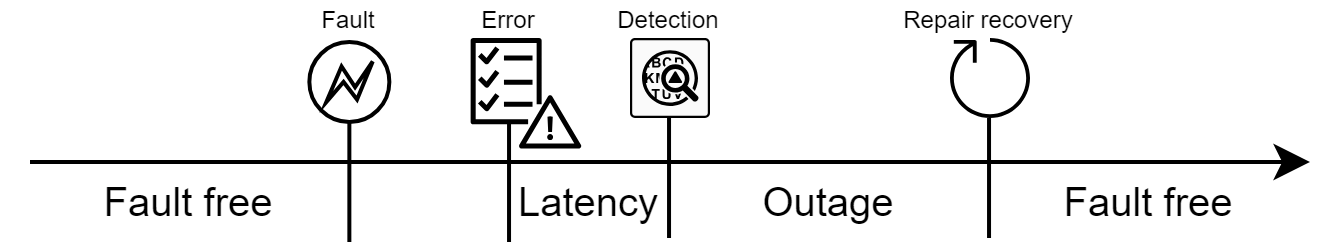
\includegraphics[width=0.75\linewidth]{images/rel.png}
    \caption{Reliability measures}
\end{figure}

\subsection{Reliability block diagrams}
Reliability block diagrams (RBDs) provide an inductive model where a system is partitioned into blocks representing distinct elements such as components or subsystems. 
Each block in the RBD has its own reliability, which can be previously calculated or modeled. 
These blocks are then combined to represent all possible success paths within the system.

Assuming that failures occur according to a Poisson model, the time between two successive failures can be modeled as follows:
\begin{itemize}
    \item Probability density function: 
        \[f(t,\lambda)=\lambda e^{-\lambda t} \qquad t\geq 0, \lambda > 0\]
    \item Cumulative density function:
        \[\text{P}(T\leq t)=\int_0^t f(s,\lambda)ds=1-e^{-\lambda t}\]
    \item Expected value: 
        \[\mathbb{E}\left[T\right]=\dfrac{1}{\lambda}\]
    \item Variance: 
        \[\sigma^2(T)=\dfrac{1}{\lambda^2}\]
\end{itemize}
As a result, reliability can be defined as:
\[R(t)=\text{P}(T \geq t)=e^{-\lambda t}\]
Here, $\lambda(t)$ represents the failure rate. 
RBDs provide an approach to compute the reliability of a system based on the reliability of its components.
\paragraph*{Reliability in series}
In the case of components arranged in series, all components must be operational for the system to function properly:
\[R_S(t)=R_{C1}(t)\cdot R_{C2}(t)\]
For systems composed of components with reliability following an exponential distribution (a common case), the Mean Time To Failure (MTTF) of the system $S$ can be expressed as:
\[\text{MTTF}_S=\dfrac{1}{\lambda_S}=\dfrac{1}{\sum_{i=1}^{n}\frac{1}{\text{MTTF}_i}}\]ì
A special case occurs when all components are identical:
\[\text{MTTF}_S=\dfrac{\text{MTTF}_1}{n}\]
\paragraph*{Availability in series}
The availability $A_S$ is calculated as:
\[A_S=\prod_{i=1}^{n}\dfrac{\text{MTTF}_i}{\text{MTTF}_i+\text{MTTR}_i}\]
When all components are identical:
\[A={\left( \dfrac{\text{MTTF}_1}{\text{MTTF}_1+\text{MTTR}_1} \right)}^n\]
\paragraph*{Reliability in parallel}
In the case of components arranged in parallel, if at least one component is operational, the system functions properly:
\[R_S(t)=R_{C1}(t)+R_{C2}(t)-R_{C1}(t)\cdot R_{C2}(t)\]
For a system $P$ composed of $n$ components: 
\[R_p(t)=1-\prod_{i=1}^{n}\left( 1-R_i(t) \right)\]
\paragraph*{Availability in parallel}
The availability $A_p$ is given by:
\[A_p(t)1-\prod_{i=1}^{n}\left(1-A_i(t)\right)\]

\paragraph*{Redundancy}
A system may consist of two parallel replicas:
\begin{itemize}
    \item The primary replica operates continuously.
    \item The redundant replica, typically disabled, is activated when the primary replica fails.
\end{itemize}
For operational redundancy, the following are necessary a mechanism to ascertain whether the primary replica is functioning correctly (online self-check), and a dynamic switching mechanism to deactivate the primary replica and activate the redundant one.
In the standby model, we calculate the system reliability using various approaches:
\begin{itemize}
    \item When failure rates are equal and switching is perfect:
        \[R_S=e^{-\lambda t}(1+\lambda t)\]
    \item In cases of unequal failure rates with perfect switching:
        \[R_S=e^{-\lambda t}+\lambda_1 \dfrac{e^{-\lambda_1 t}-e^{-\lambda_2 t}}{\lambda_2-\lambda_1}\]
    \item When failure rates are equal, but switching is imperfect:
        \[R_S=e^{-\lambda t}(1+R_V\lambda t)\]
    \item For unequal failure rates with imperfect switching:
        \[R_S=e^{-\lambda t}+R_V\lambda_1 \dfrac{e^{-\lambda_1 t}-e^{-\lambda_2 t}}{\lambda_2-\lambda_1}\]
\end{itemize}
In these equations, $R_S$ represents the system reliability, $\lambda$ stands for the failure rate, $t$ denotes the opening time, and $R_V$ indicates the switching reliability.

In a broader context, a system with one primary replica and $n$ redundant replicas (identical and perfectly switchable) can be represented by the reliability function:
\[R(t)=e^{-\lambda t}\sum_{i=0}^{n-1}\dfrac{{\left(\lambda t\right)}^i}{i!}\]
For a system comprising $n$ identical replicas where at least $r$ replicas must function correctly for the entire system to operate correctly. 
In this case we the reliability is computed as: 
\[R_S(t)=R_V\sum_{i=r}^{n}R_C^i{(1-R_C)}^{n-i}\dfrac{n!}{i!(n-i)!}\]
Here, $R_S$ represents the system reliability, $R_C$ denotes the component reliability, $R_V$ signifies the voter reliability, $n$ stands for the number of components, and $r$ indicates the minimum number of components required to remain operational.

\paragraph*{Triple modular redundancy}
Considering triple modular redundancy where 2 out of 3 components function properly, and the voter works properly:
\[\text{MTTF}_{TMR}=\dfrac{5}{6}\text{MTTR}_{simplex}\]
Thus, $\text{MTTF}_{TMR}$ is shorter than ${MTTR}_{simplex}$, allowing tolerance for transient and permanent faults, leading to higher reliability for shorter missions.

Redundancy proves beneficial when $R_{TMR}(t)>R_C(t)$ for mission times shorter than 70\% of  $\text{MTTF}_C$.
Hence, redundancy is advantageous for specific mission durations.